%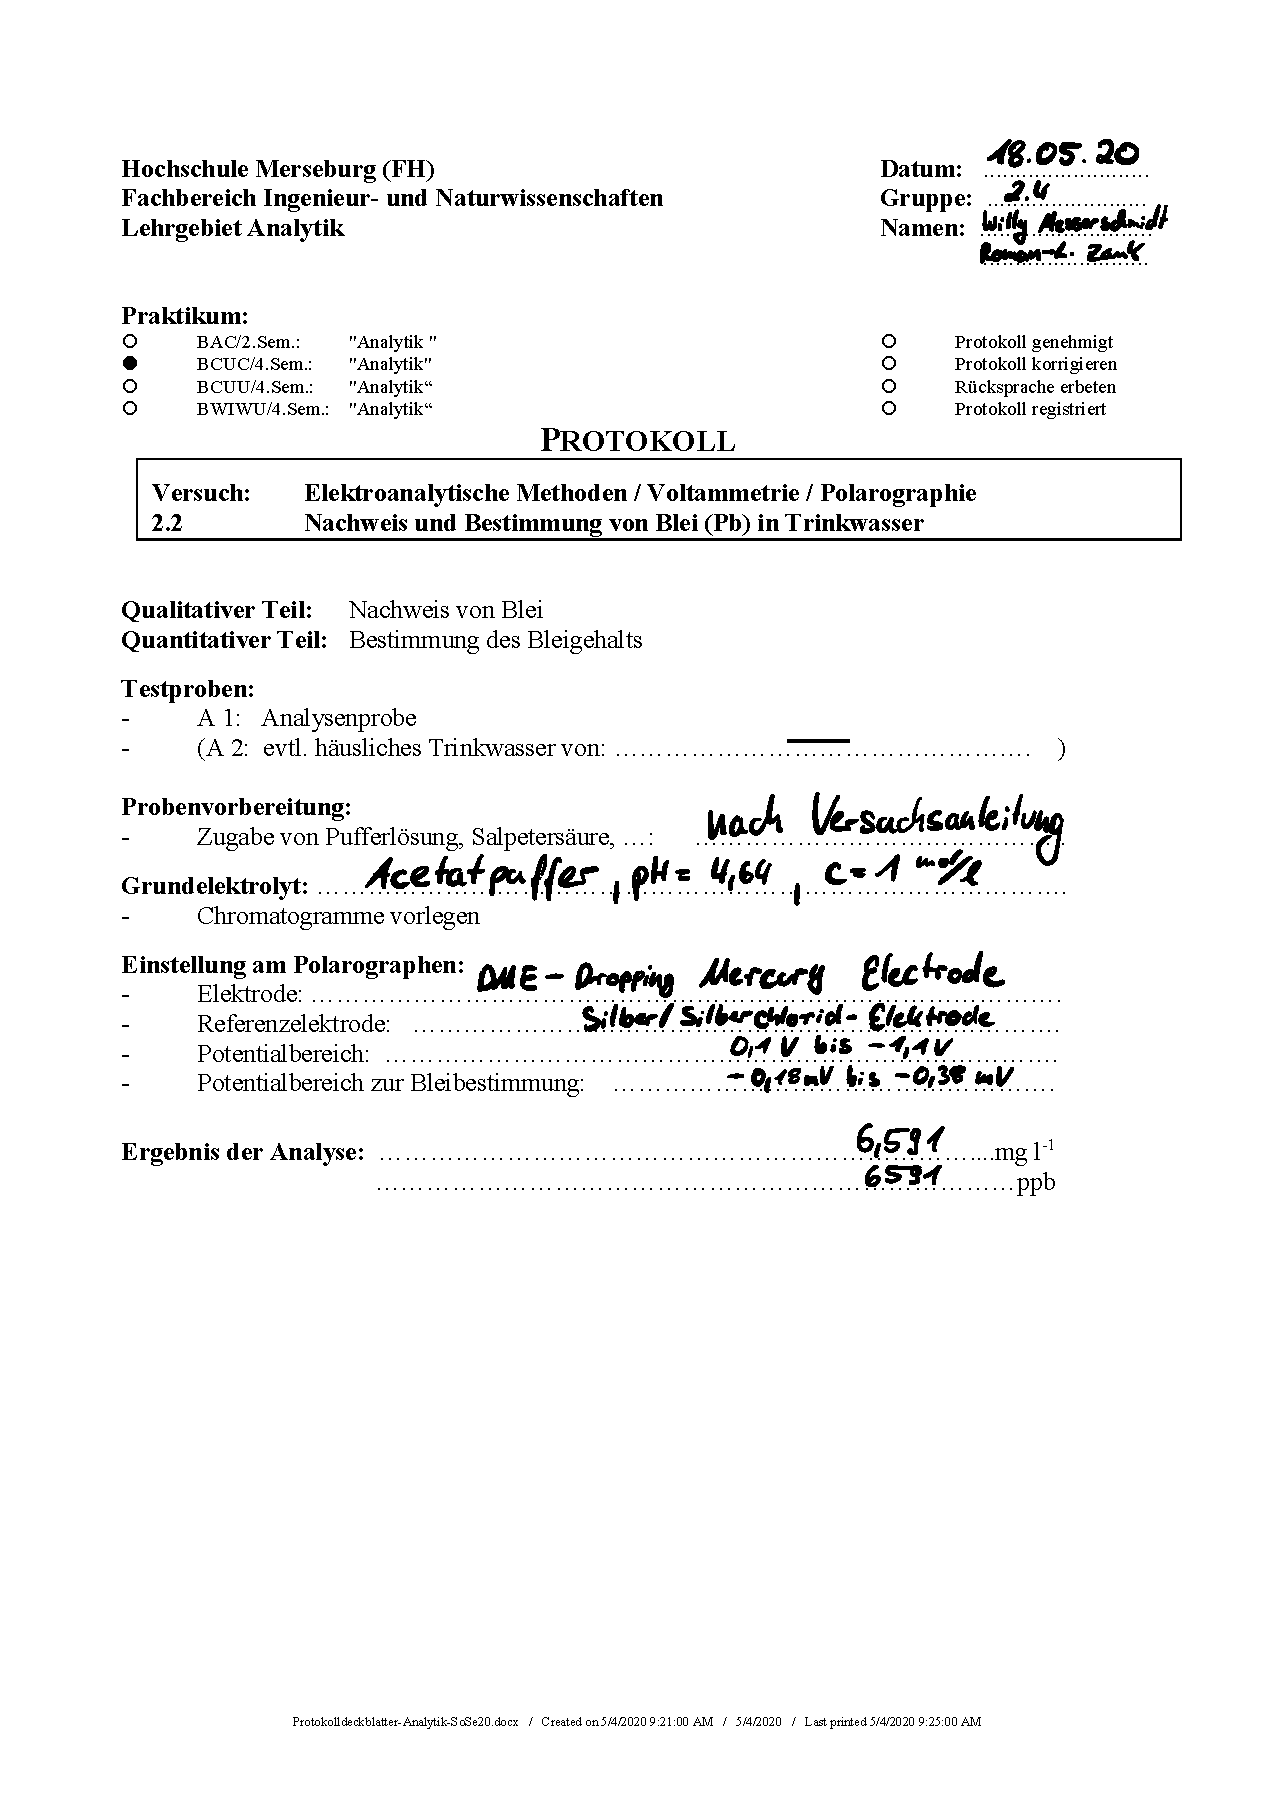
\includepdf[]{Deckblatt}
\pagebreak
\section{Einleitung}
\label{sec:einleitung}
Der Wassergehalt von flüssigen und festen Werk-, Betriebs- und Hilfsstoffen muss für ihre technische Anwendung in vielen Bereichen gemessen werden. Ein Bestimmungsverfahren stellt dabei die \textsc{Karl-Fischer}-Titration dar. Im Verlauf des hier beschriebenen Praktikumsversuches wurde eine Flüssigkeitsprobe und eine Feststoffprobe analysiert.





